\documentclass[12pt,a4paper]{report}

% ---------- Paket dasar ----------
\usepackage[utf8]{inputenc}
\usepackage[T1]{fontenc}
\usepackage[indonesian]{babel}
\usepackage{lipsum}

% ---------- Paket matematika & gambar ----------
\usepackage{amsmath,amssymb}
\usepackage{graphicx}
\usepackage{caption}
\usepackage{subcaption}
\usepackage{float}
\usepackage{algorithm}
\usepackage{algpseudocode}
\bibliographystyle{IEEEtran}
% ---------- Paket lain ----------
\usepackage[most]{tcolorbox}
\usepackage{forest}
\usepackage{hyperref}
\usepackage{fancyhdr}

% Environment pseudocode bergaya IEEE dengan bingkai,
% non-float agar dapat terpecah ke halaman berikutnya.
\newenvironment{ieeealgorithm}[1]{%
	\refstepcounter{algorithm}%
	\begin{tcolorbox}[
		enhanced,
		breakable,
		colback=white,
		colframe=black,
		colbacktitle=black,
		boxrule=0.6pt,
		title={Algorithm \thealgorithm: #1},
		fonttitle=\bfseries,
		coltitle=white,
		left=1mm,
		right=1mm,
		top=0.7mm,
		bottom=0.7mm
	]
	\begin{algorithmic}[1]
}{%
	\end{algorithmic}
	\end{tcolorbox}
}

\usepackage{titlesec}

\usepackage{titlesec}
\usepackage{longtable}
\usepackage{array} % untuk menentukan lebar kolom
\usepackage{booktabs} % gaya tabel lebih elegan
\usepackage[table]{xcolor}



% Tambah jarak aman dari header dan footer:	
\setlength{\headheight}{10pt}   % wajib cukup besar untuk fancyhdr
\setlength{\headsep}{55pt}      % jarak header ke teks
\setlength{\footskip}{28pt}     % jarak teks ke footer
\usepackage[a4paper,top=3cm,bottom=3cm,left=3cm,right=3cm]{geometry}

% Semua gambar dari folder public dan subfoldernya
\graphicspath{{public/}{public/01-pendahuluan/}{public/02-dasar-teori/}{public/03-implementasi/}}

% --- Pengaturan header & footer ---
\pagestyle{fancy}
\fancyhf{} % clear all

% --- Paksa semua halaman (termasuk awal chapter) memakai fancy ---
\fancypagestyle{plain}{%
	\fancyhf{}%
	\fancyhead[L]{%
		
\includegraphics[height=1.1cm]{logo-itb}\hspace{0.3cm}%
		
\includegraphics[height=1.1cm]{logo-stei}\hspace{0.3cm}%
	}%
	\fancyhead[R]{%
		\begin{minipage}{9cm}
			\raggedleft\bfseries IF2211 Strategi Algoritma\\
			\normalsize Laporan Akhir Tugas Besar 2\\
			Semester 2 2025/2026
		\end{minipage}
	}%
	\renewcommand{\headrulewidth}{0.4pt}%
	\fancyfoot[L]{\small v1.0}%
	\fancyfoot[C]{\small Halaman \thepage}%
	\fancyfoot[R]{\small }%
	\renewcommand{\footrulewidth}{0.4pt}%
}


\fancyhead[L]{%
	
\includegraphics[height=1.5cm]{logo-itb}\hspace{0.3cm}%
	
\includegraphics[height=1.5cm]{logo-stei}\hspace{0.3cm}%
}

\fancyhead[R]{%
	\begin{minipage}{9cm}
		\raggedleft\bfseries IF2211 Strategi Algoritma\\
		\normalsize Laporan Akhir Tugas Besar 2\\
		\itshape Semester 2 2025/2026
	\end{minipage}
}

\renewcommand{\headrulewidth}{0.4pt}

\fancyfoot[L]{\small v1.0}
\fancyfoot[C]{\small Halaman \thepage}
\fancyfoot[R]{\small }
\renewcommand{\footrulewidth}{0.4pt}

\begin{document}

\begin{titlepage}
	\thispagestyle{empty}
	\centering

	% ---------- Judul utama ----------
	{\LARGE \textbf{Tugas Besar 2}\par}
	\vspace{0.2cm}
	{\LARGE \textbf{nama\_kelompok}\par}
	\vspace{0.8cm}
	{\large IF2211 Strategi Algoritma\par}
	\vspace{0.2cm}
	{\large DOMTracer : BFS-DFS Based CSS Selector Engine\par}
	\vspace{0.2cm}
	{\large Semester 2 2025/2026\par}

	% ---------- Gambar tengah ----------
	\vspace{1.8cm}
	
\includegraphics[width=0.9\textwidth]{foto-kelompok}\par

	% ---------- Disusun oleh ----------
	\vspace{1.2cm}
	{\bfseries Disusun oleh:\par}
	\vspace{0.2cm}
	\textbf{nama\_kelompok}
	\vspace{0.5cm} \\
	\begin{tabular}{l l}
		Moh. Hafizh Irham Perdana   & (13524025) \\
		Aufa Rienaldifaza Ahmad     & (13524027) \\
		Muhammad Aufar Rizqi Kusuma & (13524061) \\
	\end{tabular}

	% ---------- Institusi ----------
	\vspace{2.0cm}
	Laboratorium Ilmu dan Rekayasa Komputasi\par
	Program Studi Teknik Informatika\par
	Sekolah Teknik Elektro dan Informatika\par
	Institut Teknologi Bandung\par

\end{titlepage}

\clearpage
\pagestyle{fancy}

\tableofcontents
\clearpage

\chapter{Pendahuluan}
\section{Deskripsi Tugas}
\begin{figure}[H]
    \centering
    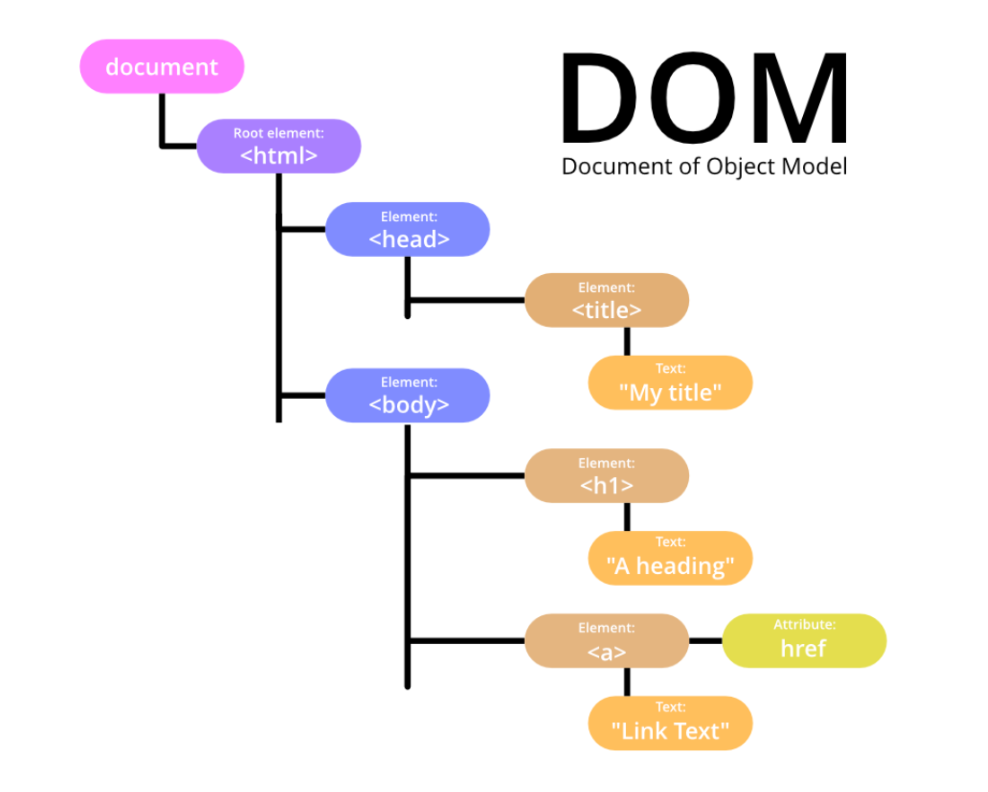
\includegraphics[width=0.7\textwidth]{01-pendahuluan/struktur-pohon.png}
    \caption{Struktur Pohon DOM}
\end{figure}
Document Object Model (DOM) merupakan representasi terstruktur dari dokumen HTML dalam bentuk tree yang memungkinkan setiap elemen pada halaman web diakses, dimodifikasi, dan dimanipulasi oleh program. Struktur ini merepresentasikan hubungan antar elemen HTML seperti parent, child, dan sibling sehingga memudahkan pengolahan dokumen secara terprogram. Struktur sebuah file HTML pada umumnya meliputi elemen root <html> yang berisi dua bagian utama yaitu <head> dan <body>. Bagian <head> berisi metadata seperti judul halaman, link stylesheet, dan script, sedangkan <body> berisi konten utama halaman seperti teks, gambar, tombol, dan elemen HTML lainnya yang ditampilkan kepada pengguna.

Sebuah website menampilkan sebuah DOM melalui sebuah file bernama Cascading Style Sheets (CSS) yang bertujuan mendeklarasikan visualisasi elemen-elemen pada pohon. Deklarasi visualisasi ditempelkan pada elemen-elemen yang berkaitan melalui CSS Selector. Pada Tugas Besar 2 Strategi Algoritma ini, mahasiswa diminta untuk menelusuri dan mencari elemen pada struktur DOM berdasarkan CSS Selector tertentu dengan menggunakan algoritma penelusuran graf yaitu Breadth First Search (BFS) dan Depth First Search (DFS). Algoritma tersebut digunakan untuk menjelajahi struktur pohon DOM guna menemukan elemen yang sesuai dengan selector yang diberikan.

Komponen-komponen penting yang terdapat pada tugas besar ini antara lain:
\begin{enumerate}
    \item \textbf{Tags} pada HTML merupakan penanda (markup) yang digunakan untuk mendefinisikan struktur dan jenis elemen dalam sebuah dokumen HTML. Tag memberi tahu browser bagaimana suatu bagian konten harus ditafsirkan dan ditampilkan pada halaman web.
          \begin{figure}[H]
              \centering
              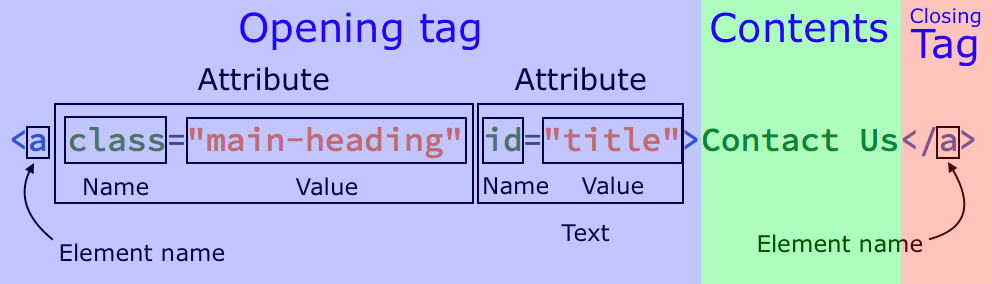
\includegraphics[width=0.7\textwidth] {01-pendahuluan/syntax-html.png}
              \caption{Struktur Pohon DOM}
          \end{figure}
          Secara umum, tag HTML ditulis menggunakan tanda kurung sudut (\texttt{<>}). Sebagian besar elemen HTML memiliki pasangan tag pembuka dan tag penutup. Tag pembuka menandai awal suatu elemen, sedangkan tag penutup menandai akhir elemen tersebut. Tag penutup ditulis dengan menambahkan tanda garis miring/sebelum nama tag. Terdapat beberapa jenis tag HTML yang self-closing.

          Dalam struktur DOM, setiap tag HTML direpresentasikan sebagai node pada pohon DOM. Hubungan antar tag membentuk struktur hierarki seperti parent, child, dan sibling. Struktur inilah yang memungkinkan dokumen HTML diproses sebagai sebuah pohon ketika dilakukan penelusuran menggunakan algoritma seperti BFS atau DFS.
    \item \textbf{CSS Selector} adalah mekanisme pada CSS untuk memilih elemen HTML tertentu pada struktur DOM agar dapat diberikan aturan style. Dengan selector, kita dapat menentukan elemen mana yang akan dikenai aturan visual seperti warna, ukuran, atau tata letak.
          \begin{figure}[H]
              \centering
              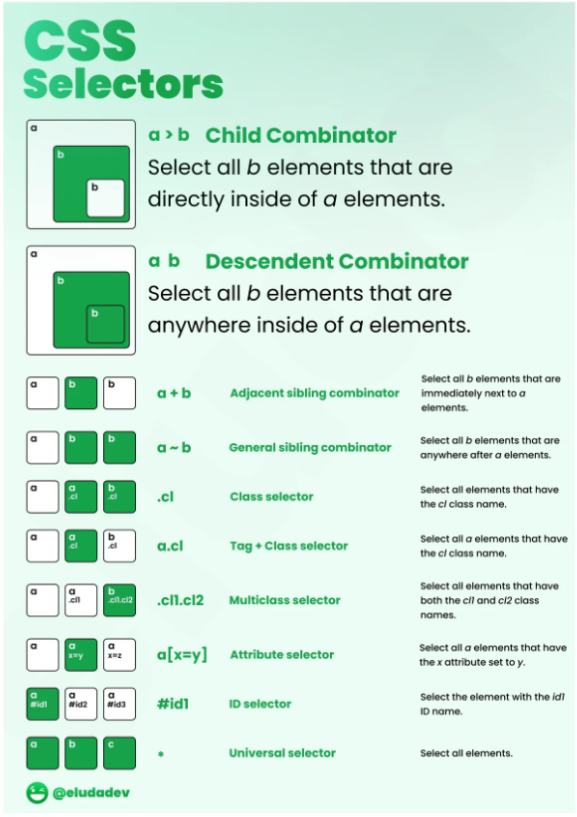
\includegraphics[width=0.4\textwidth] {01-pendahuluan/css-selector.png}
              \caption{Struktur Pohon DOM}
          \end{figure}

          Beberapa selector dasar yang umum digunakan adalah sebagai berikut.
          \begin{enumerate}
              \item \textbf{Tag Selector}. Memilih elemen berdasarkan nama tag HTML. Contoh: \texttt{p} memilih semua elemen \texttt{<p>}.
              \item \textbf{Class Selector}. Memilih elemen yang memiliki atribut class tertentu, ditulis dengan tanda titik (.). Contoh: \texttt{.box}.
              \item \textbf{ID Selector}. Memilih elemen dengan atribut id tertentu, ditulis dengan tanda pagar (\#). Contoh: \texttt{\#header}
              \item \textbf{Universal Selector}. Memilih semua elemen HTML. Contoh: *.
          \end{enumerate}
          Combinator merupakan cara untuk menggabungkan beberapa jenis selector dalam penentuan elemen yang akan terpengaruh, dan terdiri dari list berikut ini.
          \begin{enumerate}
              \item Child Combinator (\texttt{>})
              \item Descendent Combinator (\texttt{“ “})
              \item Adjacent Sibling Combinator (\texttt{+})
              \item General Sibling Combinator (\texttt{~})
          \end{enumerate}

    \item \textbf{HTML Parsing} adalah Proses membaca dokumen HTML dan mengubahnya menjadi struktur data pohon (tree) yang merepresentasikan hubungan antar elemen HTML. Pada proses ini, parser memproses dokumen HTML secara berurutan, mengenali tag pembuka dan tag penutup, kemudian menyusunnya ke dalam struktur hierarki.
          \begin{figure}[H]
              \centering
              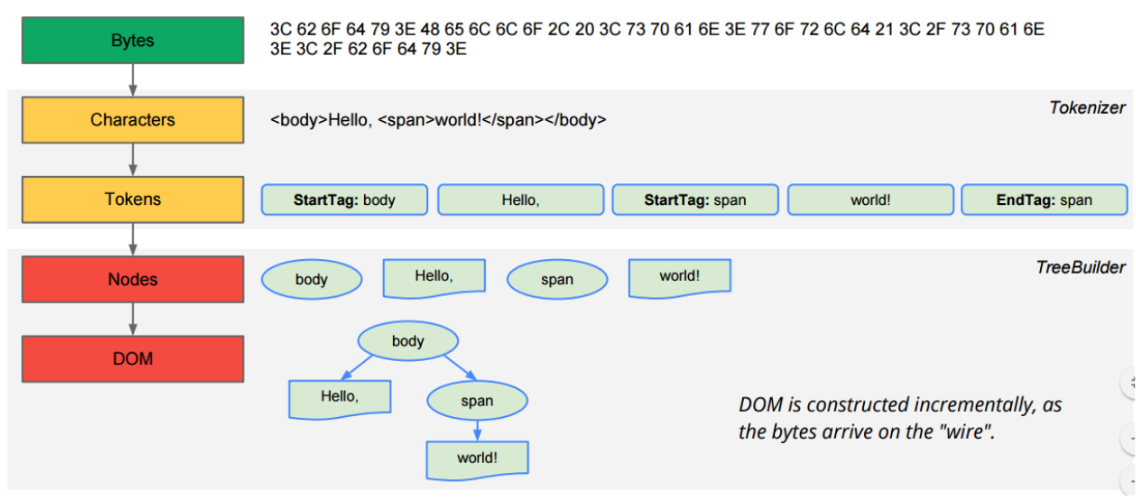
\includegraphics[width=0.4\textwidth] {01-pendahuluan/parsing-html.png}
              \caption{Struktur Pohon DOM}
          \end{figure}

          Setiap tag HTML direpresentasikan sebagai node pada pohon. Tag yang berada di dalam tag lain akan menjadi child node, sedangkan tag yang membungkusnya menjadi parent node. Node paling atas pada struktur ini disebut root, yang umumnya merupakan elemen <html>. Dari node root tersebut, elemen-elemen lain seperti \texttt{<head>} dan \texttt{<body>} akan menjadi cabang yang membentuk struktur pohon DOM.

          Hasil dari proses parsing adalah DOM Tree, yaitu representasi pohon dari dokumen HTML yang memungkinkan elemen-elemen pada halaman web ditelusuri, diakses, dan dimanipulasi secara terstruktur. Struktur pohon ini kemudian dapat digunakan dalam proses penelusuran elemen, misalnya dengan menggunakan algoritma Breadth First Search (BFS) atau Depth First Search (DFS).
\end{enumerate}

\section{Spesifikasi Wajib}
Pada tugas ini, mahasiswa diminta untuk membuat aplikasi traversal pohon HTML (DOM Tree) yang menggunakan algoritma Breadth First Search (BFS) dan Depth First Search (DFS) untuk melakukan pencarian elemen berdasarkan CSS selector pada struktur DOM.
\begin{itemize}
    \item Buatlah sebuah aplikasi berbasis web yang terdiri dari frontend bebas dan backend dalam bahasa Go, C\#, Rust, atau Typescript yang mengimplementasikan algoritma BFS dan DFS untuk melakukan penelusuran CSS pada pohon DOM.
    \item Aplikasi dapat melakukan scraping HTML dari sebuah website melalui URL yang diberikan oleh pengguna.
    \item Secara umum, berikut adalah input yang diharapkan.
          \begin{itemize}
              \item URL website atau memasuki teks HTML sendiri
              \item Pilihan algoritma traversal (BFS / DFS)
              \item CSS selector
              \item Jumlah hasil yang diinginkan:
                    \begin{itemize}
                        \item Top \textit{n} kemunculan
                        \item Semua kemunculan
                    \end{itemize}
          \end{itemize}
    \item HTML yang diperoleh kemudian diparsing menjadi struktur data pohon (DOM Tree).
    \item Output yang diharapkan adalah sebagai berikut.
          \begin{enumerate}
              \item Aplikasi dapat menampilkan visualisasi struktur pohon DOM, disertai dengan keterangan kedalaman maksimum tree.
              \item Aplikasi dapat menampilkan highlight pada jalur yang di-traversal oleh algoritma penelusuran yang dipilih untuk menandakan elemen-elemen yang terpengaruh.
              \item Aplikasi dapat menampilkan waktu pencarian serta banyak node yang dikunjungi.
              \item Setelah melakukan penelusuran, aplikasi menyimpan sebuah traversal log yang memiliki informasi tahapan penelusuran yang dilakukan.
          \end{enumerate}
    \item Repository bagian frontend dan backend boleh digabung/dipisah.
    \item Setiap kelompok harap mengisi nama kelompok dan anggotanya pada link berikut, dengan maksimal tanggal Minggu, 5 April 2026 2026 23.59. Nama kelompok dilarang mengandung unsur SARA, penghinaan, provokasi, atau hal-hal lain yang bertentangan dengan norma hukum.
    \item Perlu diperhatikan bahwa kelompok tubes untuk mata kuliah ini tidak boleh sama. Jadi jika berkelompok dengan X pada tubes ini, maka pada tubes selanjutnya anda tidak diperkenankan berkelompok dengan X.
\end{itemize}

\section{Spesifikasi Bonus}
\begin{itemize}
    \item \textbf{(4 poin) [Video]} Membuat video tentang aplikasi BFS dan DFS pada penelusuran pohon DOM kemudian mengunggahnya di Youtube. Video dibuat harus memiliki audio dan menampilkan wajah dari setiap anggota kelompok. Untuk contoh video tubes stima tahun-tahun sebelumnya dapat dilihat di Youtube dengan kata kunci “Tubes Stima”, “strategi algoritma”, “Tugas besar stima”, dll. Semakin menarik video, maka semakin banyak poin yang diberikan.
    \item \textbf{(5 poin) [Deploy]} Aplikasi web yang telah dibuat perlu di deploy menggunakan Microsoft Azure Virtual Machine (VM) sehingga aplikasi dapat diakses secara publik melalui internet. Sebagai mahasiswa, terdapat kredit gratis sebesar \$100 dari Microsoft untuk dapat digunakan hanya dengan menggunakan email kampus ITB. Karena layanan ini menggunakan sistem pembayaran berbasis penggunaan (pay-as-you-go), penggunaan Virtual Machine akan mengurangi kredit yang dimiliki. Oleh karena itu, disarankan untuk mematikan (stop/deallocate) Virtual Machine ketika tidak digunakan agar kredit Azure tidak cepat habis.
    \item \textbf{(2 Poin) [Docker]} Aplikasi dijalankan menggunakan Docker baik untuk frontend maupun backend.
    \item \textbf{(6 Poin) [Animasi]} Menampilkan animasi penelusuran pohon DOM untuk segala pencarian.
    \item \textbf{(3 Poin) [Multithreading]} Mengimplementasikan multithreading pada algoritma BFS dan/atau DFS untuk melakukan traversal pohon DOM secara paralel. Proses traversal dibagi ke beberapa thread/worker sehingga beberapa node dapat diproses secara bersamaan.
    \item \textbf{(3 Poin) [LCA Binary Lifting]} Mengimplementasikan algoritma Lowest Common Ancestor (LCA) dengan teknik Binary Lifting pada pohon DOM yang dihasilkan dari proses parsing HTML. LCA digunakan untuk menentukan node leluhur terendah yang sama dari dua node dalam sebuah pohon. Dalam konteks DOM, fitur ini dapat digunakan untuk mengetahui elemen HTML terdekat yang menjadi parent bersama dari dua elemen tertentu. Penjelasan lebih lanjut dapat dilihat pada link berikut.
\end{itemize}

\chapter{Dasar Teori}
\section{Document Object Model}

Document Object Model (DOM) adalah representasi dokumen HTML dalam bentuk struktur pohon yang dapat diakses oleh program. Setiap elemen HTML direpresentasikan sebagai node, sedangkan hubungan antarelemen direpresentasikan sebagai relasi \textit{parent}, \textit{child}, dan \textit{sibling}. Pada konteks tugas ini, DOM menjadi model data utama karena proses pencarian elemen berdasarkan CSS selector dapat dipandang sebagai penelusuran node pada pohon berakar \cite{whatwgdom}.

Sebuah pohon DOM memiliki satu akar utama, umumnya elemen \texttt{html}. Di bawah akar tersebut terdapat subtree seperti \texttt{head} dan \texttt{body}, lalu elemen-elemen lain yang bersarang di dalamnya. Informasi yang penting untuk pencarian meliputi nama tag, atribut, teks, daftar anak, parent, dan kedalaman node. Kedalaman dipakai untuk mengetahui posisi node terhadap root, sedangkan jalur dari root ke node dapat digunakan untuk menampilkan rute hasil pencarian pada antarmuka aplikasi.

\section{HTML Parsing}

HTML parsing adalah proses mengubah dokumen HTML mentah menjadi struktur DOM yang terorganisasi. Parser membaca token HTML seperti \textit{start tag}, \textit{end tag}, teks, dan \textit{self-closing tag}, lalu menyusun token tersebut menjadi pohon sesuai aturan penyarangan elemen HTML \cite{whatwghtml}. Dalam implementasi aplikasi, tahap ini diperlukan sebelum BFS atau DFS dijalankan karena algoritma traversal membutuhkan struktur node dan relasi parent-child yang eksplisit.

Salah satu pendekatan umum untuk membangun pohon dari token HTML adalah menggunakan stack. Ketika parser menemukan tag pembuka, node baru dibuat sebagai anak dari node pada puncak stack, kemudian node tersebut dimasukkan ke stack jika bukan elemen kosong. Ketika tag penutup ditemukan, stack dipop hingga tag yang sesuai ditemukan. Untuk tag kosong seperti \texttt{img}, \texttt{br}, \texttt{meta}, atau \texttt{input}, node tetap dimasukkan ke pohon tetapi tidak menjadi parent aktif. Pendekatan ini efisien karena dokumen dapat diproses secara linear terhadap panjang input.

\section{CSS Selector}

CSS selector adalah pola yang digunakan untuk memilih elemen HTML tertentu. Dalam CSS, selector berfungsi menghubungkan aturan gaya dengan elemen target; dalam aplikasi ini, selector digunakan sebagai predikat pencarian terhadap node DOM \cite{w3cselectors}. Sebuah node dianggap cocok apabila tag, atribut, atau relasi strukturalnya memenuhi selector yang diberikan pengguna.

Selector sederhana yang relevan dengan implementasi terdiri atas tag selector, class selector, id selector, dan universal selector. Tag selector memilih node berdasarkan nama tag, misalnya \texttt{article}. Class selector memilih node yang memiliki class tertentu, misalnya \texttt{.product\_pod}. ID selector memilih node dengan atribut \texttt{id} tertentu, misalnya \texttt{\#main}. Universal selector \texttt{*} memilih semua node.

Selain selector sederhana, CSS juga mengenal combinator untuk menyatakan relasi antarnode. Descendant combinator \texttt{A B} memilih node \texttt{B} yang memiliki ancestor \texttt{A}. Child combinator \texttt{A > B} memilih node \texttt{B} yang parent langsungnya adalah \texttt{A}. Adjacent sibling combinator \texttt{A + B} memilih node \texttt{B} yang muncul tepat setelah sibling \texttt{A}. General sibling combinator \texttt{A \textasciitilde{} B} memilih node \texttt{B} yang muncul setelah sibling \texttt{A} pada parent yang sama. Keempat relasi ini sesuai dengan informasi struktural yang tersedia pada pohon DOM.

\section{Traversal Graf pada Pohon DOM}

Pohon DOM dapat dipandang sebagai graf terhubung tanpa siklus dengan satu root. Oleh karena itu, pencarian elemen pada DOM dapat dilakukan dengan algoritma traversal graf. Dua strategi traversal yang digunakan pada tugas ini adalah Breadth-First Search (BFS) dan Depth-First Search (DFS). Keduanya mengunjungi node-node pada pohon dan mengevaluasi selector pada setiap node, tetapi memiliki urutan kunjungan yang berbeda \cite{cormen2009introduction}.

\subsection{Breadth-First Search}

Breadth-First Search menelusuri pohon secara melebar dari root. Node pada kedalaman yang lebih kecil dikunjungi lebih dahulu sebelum node pada kedalaman berikutnya. Secara umum, BFS menggunakan struktur data queue dengan prinsip FIFO (\textit{First In, First Out}). Pada DOM, BFS cocok digunakan ketika elemen target diperkirakan berada dekat dengan root atau ketika urutan hasil berdasarkan level pohon lebih diinginkan.

Jika jumlah node adalah $N$, kompleksitas waktu BFS adalah $O(N)$ karena setiap node dikunjungi paling banyak satu kali. Kompleksitas ruangnya bergantung pada lebar maksimum pohon, yaitu $O(W)$, karena queue dapat menyimpan banyak node pada level yang sama. Dalam pencarian berbasis selector, biaya total dapat ditulis sebagai $O(N \cdot C)$, dengan $C$ sebagai biaya evaluasi selector pada satu node.

\subsection{Depth-First Search}

Depth-First Search menelusuri pohon secara mendalam. Algoritma ini mengunjungi satu cabang sampai sejauh mungkin, lalu kembali untuk memproses cabang lain. DFS dapat diimplementasikan secara rekursif atau iteratif menggunakan stack dengan prinsip LIFO (\textit{Last In, First Out}). Pada DOM, DFS cocok untuk mengeksplorasi subtree yang dalam karena traversal segera masuk ke anak sebuah node sebelum berpindah ke sibling berikutnya.

Sama seperti BFS, kompleksitas waktu DFS adalah $O(N)$ untuk mengunjungi seluruh node. Kompleksitas ruang DFS iteratif bergantung pada tinggi pohon dan jumlah node yang tersimpan pada stack, sehingga pada pohon yang relatif seimbang dapat mendekati $O(H)$, dengan $H$ sebagai tinggi pohon. Pada kasus terburuk, ruang yang digunakan tetap dapat mencapai $O(N)$.

\section{Pencarian Elemen dan Metrik Traversal}

Pencarian elemen pada aplikasi ini dilakukan dengan menggabungkan traversal dan selector matching. Traversal menentukan urutan node yang dikunjungi, sedangkan selector menentukan apakah node tersebut masuk ke daftar hasil. Karena BFS dan DFS memakai predikat selector yang sama, himpunan hasil untuk pencarian tanpa limit seharusnya sama; perbedaannya terletak pada urutan hasil, traversal log, dan jumlah node yang dikunjungi sebelum berhenti ketika fitur Top-$N$ digunakan.

Beberapa metrik penting yang digunakan untuk mengevaluasi pencarian adalah jumlah node yang dikunjungi, jumlah node yang cocok, kedalaman maksimum yang dijangkau, waktu eksekusi, dan status berhenti karena limit. Jumlah node yang dikunjungi menunjukkan besar area DOM yang dieksplorasi. Kedalaman maksimum membantu menggambarkan seberapa jauh traversal masuk ke struktur dokumen. Waktu eksekusi digunakan untuk membandingkan efisiensi praktis BFS dan DFS pada selector serta dokumen yang sama. Traversal log menyimpan urutan kunjungan node sehingga proses pencarian dapat divisualisasikan kembali pada frontend.

\section{Aplikasi Web dan Pertukaran Data}

Aplikasi tugas besar ini memisahkan pemrosesan utama pada backend dan visualisasi pada frontend. Backend bertugas mengambil atau menerima HTML, melakukan parsing, menjalankan BFS atau DFS, mengevaluasi selector, dan mengembalikan hasil dalam format JSON. Frontend bertugas menyediakan masukan pengguna, menampilkan pohon DOM, menyorot hasil pencarian, serta menyajikan metrik dan log traversal.

Format JSON sesuai untuk pertukaran data karena struktur node, atribut, daftar anak, hasil pencarian, dan log traversal dapat direpresentasikan secara hierarkis. Dengan demikian, pohon DOM yang diproses di backend dapat divisualisasikan kembali oleh frontend tanpa kehilangan informasi penting seperti tag, atribut, teks, kedalaman, path node, dan status kecocokan selector.


\chapter{Aplikasi BFS dan DFS}
\section{Pendekatan Umum}

Pendekatan utama pada aplikasi ini berfokus pada dua strategi traversal pohon DOM, yaitu Breadth-First Search (BFS) dan Depth-First Search (DFS). Sebelum traversal dijalankan, masukan HTML terlebih dahulu diparse menjadi pohon DOM agar setiap elemen memiliki relasi parent-child yang jelas. Setelah struktur pohon terbentuk, selector CSS dipakai sebagai filter untuk menentukan node mana yang dianggap cocok selama proses penelusuran.

Pada BFS, penelusuran dilakukan per level menggunakan queue (FIFO), sehingga node yang lebih dekat ke akar diproses lebih dahulu. Karakter ini membuat BFS cocok ketika tujuan utama adalah menemukan elemen yang berada pada kedalaman dangkal atau ketika urutan hasil berdasarkan level lebih diutamakan. Selama traversal, setiap node yang dikunjungi tetap dievaluasi terhadap selector, sehingga hasil tidak hanya bergantung pada urutan kunjungan, tetapi juga pada kecocokan kriterianya.

Pada DFS, penelusuran dilakukan sedalam mungkin pada satu cabang menggunakan stack (LIFO), lalu melakukan backtrack ke cabang lain. Pendekatan ini cocok untuk eksplorasi struktur yang dalam karena sistem segera masuk ke subtree sebelum berpindah ke sibling berikutnya. Seperti pada BFS, selector tetap dievaluasi di setiap langkah agar hanya node yang memenuhi kriteria yang dicatat sebagai match.

Perbedaan inti BFS dan DFS pada implementasi ini terletak pada urutan kunjungan node, jejak traversal, serta kemungkinan waktu tercapainya limit hasil. Meskipun urutan temuan dapat berbeda, keduanya menggunakan aturan selector yang sama dan menghasilkan keluaran dalam format metrik yang sama, seperti jumlah node dikunjungi, kedalaman maksimum, dan durasi eksekusi.

\section{Parsing}

Parsing pada program ini bertujuan mengubah dokumen HTML mentah menjadi representasi pohon DOM yang dapat ditelusuri oleh BFS maupun DFS. Tahap ini menjadi fondasi karena kualitas hasil traversal sangat bergantung pada ketepatan struktur parent-child yang dibentuk saat parsing. Implementasi di backend menggunakan tokenizer HTML berbasis stream dari pustaka \texttt{golang.org/x/net/html}, sehingga dokumen dibaca token per token tanpa perlu membangun representasi string antara yang besar di memori.

Pendekatan yang dipakai adalah kombinasi \textit{token stream processing} dan \textit{stack-based tree construction}. Program membuat node akar semu \texttt{document} dengan kedalaman \texttt{-1}, lalu memelihara stack elemen aktif untuk menentukan parent dari token yang sedang diproses. Ketika menemukan \texttt{StartTagToken}, parser membuat node baru, menyalin atribut dari tokenizer, menautkan node tersebut ke parent pada puncak stack, dan mendorongnya ke stack jika tag bukan \textit{self-closing}. Ketika menemukan \texttt{TextToken}, isi teks dibersihkan dengan \texttt{TrimSpace}; jika tidak kosong, teks disimpan pada node yang sedang aktif. Ketika menemukan \texttt{EndTagToken}, stack dipop sampai tag yang sesuai ditemukan sehingga parser tetap toleran terhadap struktur penutup yang tidak rapi. Untuk \texttt{SelfClosingTagToken}, node tetap dibuat dan ditautkan ke parent, tetapi tidak didorong ke stack. Saat \texttt{ErrorToken} mencapai \texttt{EOF}, parser mengembalikan elemen akar HTML pertama sebagai root hasil parsing.

\subsection{Pseudocode Algoritma Parsing}

\begin{ieeealgorithm}{ParseHTML}
    \Require \texttt{rawHTML} berupa string HTML
    \Ensure \texttt{rootNode} atau \texttt{error}
    \State \texttt{tokenizer} $\gets$ \textsc{NewHTMLTokenizer}(\texttt{rawHTML})
    \State \texttt{sentinel} $\gets$ Node(tag = \texttt{"document"}, depth = $-1$)
    \State \texttt{stack} $\gets$ [\texttt{sentinel}]
    \While{true}
    \State \texttt{tokenType} $\gets$ \texttt{tokenizer.Next()}
    \If{\texttt{tokenType} = ErrorToken}
    \If{\texttt{tokenizer.Err()} = EOF}
    \If{\texttt{sentinel.children} tidak kosong}
    \State \Return \texttt{sentinel.children[0]}
    \Else
    \State \Return \texttt{error("empty document")}
    \EndIf
    \EndIf
    \ElsIf{\texttt{tokenType} = StartTagToken}
    \State \texttt{tag, hasAttr} $\gets$ \texttt{tokenizer.TagName()}
    \State \texttt{attrs} $\gets$ \textsc{ExtractAttributes}(\texttt{tokenizer}, \texttt{hasAttr})
    \State \texttt{parent} $\gets$ \texttt{top(stack)}
    \State \texttt{node} $\gets$ Node(tag = \texttt{tag}, attrs = \texttt{attrs}, parent = \texttt{parent}, depth = $|stack|-1$)
    \State tambahkan \texttt{node} ke \texttt{parent.children}
    \If{\texttt{tag} bukan anggota \texttt{SelfClosingTagSet}}
    \State \texttt{push(stack, node)}
    \EndIf
    \ElsIf{\texttt{tokenType} = TextToken}
    \State \texttt{txt} $\gets$ \textsc{TrimSpace}(\texttt{tokenizer.Text()})
    \If{\texttt{txt} $\neq$ \texttt{""}}
    \State \texttt{top(stack).text} $\gets$ \texttt{txt}
    \EndIf
    \ElsIf{\texttt{tokenType} = EndTagToken}
    \State \texttt{closingTag} $\gets$ \texttt{tokenizer.TagName()}
    \While{$|stack| > 1$}
    \State \texttt{topNode} $\gets$ \texttt{pop(stack)}
    \If{\texttt{topNode.tag} = \texttt{closingTag}}
    \State \textbf{break}
    \EndIf
    \EndWhile
    \ElsIf{\texttt{tokenType} = SelfClosingTagToken}
    \State \texttt{tag, hasAttr} $\gets$ \texttt{tokenizer.TagName()}
    \State \texttt{attrs} $\gets$ \textsc{ExtractAttributes}(\texttt{tokenizer}, \texttt{hasAttr})
    \State \texttt{parent} $\gets$ \texttt{top(stack)}
    \State \texttt{node} $\gets$ Node(tag = \texttt{tag}, attrs = \texttt{attrs}, parent = \texttt{parent}, depth = $|stack|-1$)
    \State tambahkan \texttt{node} ke \texttt{parent.children}
    \EndIf
    \EndWhile
\end{ieeealgorithm}

\begin{ieeealgorithm}{ExtractAttributes}
    \Require \texttt{tokenizer}, \texttt{hasAttr}
    \Ensure \texttt{attrs} berupa map key-value atribut
    \State \texttt{attrs} $\gets$ map kosong
    \If{\texttt{hasAttr} = false}
    \State \Return \texttt{attrs}
    \EndIf
    \Repeat
    \State \texttt{key, value, more} $\gets$ \texttt{tokenizer.TagAttr()}
    \State \texttt{attrs[key]} $\gets$ \texttt{value}
    \Until{\texttt{more} = false}
    \State \Return \texttt{attrs}
\end{ieeealgorithm}

\subsection{Jenis File HTML yang Dapat Dimasukkan}

Program menerima masukan HTML dari tiga sumber, yaitu URL (melalui HTTP GET), berkas lokal, dan string HTML manual. Untuk berkas lokal, ekstensi yang umum seperti \texttt{.html} dan \texttt{.htm} dapat diproses selama kontennya valid sebagai dokumen HTML teks. Karena parsing menggunakan tokenizer HTML5 yang toleran, dokumen dengan struktur tidak sepenuhnya rapi seperti tag yang tidak tertutup sempurna tetap dapat diparse dalam banyak kasus. Implementasi juga mendukung elemen \textit{void/self-closing} populer seperti \texttt{img}, \texttt{br}, \texttt{hr}, \texttt{input}, \texttt{meta}, \texttt{link}, dan sejenisnya. Sebaliknya, parser ini tidak menargetkan semantik XML ketat atau kebutuhan namespace khusus, sehingga fokusnya tetap pada HTML web umum untuk kebutuhan traversal selector.

\subsection{Contoh Masukan dan Keluaran Parsing}

Contoh pertama memperlihatkan masukan sederhana dengan elemen bertingkat dan atribut. Setelah diparse, keluaran berupa node root \texttt{html} beserta subtree lengkapnya.

\begin{tcblisting}{
        breakable,
        colback=gray!3,
        colframe=black!60,
        title=Contoh 1: Input dan Output Parsing,
        listing only,
        left=1mm,
        right=1mm,
        top=1mm,
        bottom=1mm
    }
    Input HTML
    <html>
    <body id="main">
    <section class="catalog">
    <article class="item featured">Alpha</article>
    <article class="item">Beta</article>
    </section>
    </body>
    </html>

    Output (ringkas)
    {
    "tag": "html",
    "depth": 0,
    "children": [
    {
    "tag": "body",
    "attributes": {"id": "main"},
    "depth": 1,
    "children": [
    {
    "tag": "section",
    "attributes": {"class": "catalog"},
    "depth": 2,
    "children": [
    {
    "tag": "article",
    "attributes": {"class": "item featured"},
    "text": "Alpha",
    "depth": 3
    },
    {
    "tag": "article",
    "attributes": {"class": "item"},
    "text": "Beta",
    "depth": 3
    }
    ]
    }
    ]
    }
    ]
    }
\end{tcblisting}

Contoh kedua menekankan penanganan elemen \textit{self-closing}. Elemen \texttt{img} tetap masuk sebagai node anak, tetapi tidak mengubah stack kedalaman karena tidak memiliki pasangan \texttt{EndTag}.

\begin{tcblisting}{
        breakable,
        colback=gray!3,
        colframe=black!60,
        title=Contoh 2: Self-Closing Tag,
        listing only,
        left=1mm,
        right=1mm,
        top=1mm,
        bottom=1mm
    }
    Input HTML
    <html>
    <body>
    <div>
    <img class="hero" />
    <p id="lead">Intro</p>
    </div>
    </body>
    </html>

    Output (ringkas)
    html(depth=0)
    body(depth=1)
    div(depth=2)
    img[class="hero"](depth=3)
    p[id="lead"] text="Intro" (depth=3)
\end{tcblisting}

Dengan pendekatan ini, hasil parsing konsisten untuk dipakai pada tahap selector matching dan traversal BFS/DFS, karena struktur pohon, atribut, teks, dan kedalaman node sudah tersedia secara eksplisit sejak awal proses.

\section{Selector}

Modul selector bertanggung jawab untuk menentukan apakah sebuah node DOM cocok dengan pola CSS selector yang dimasukkan pengguna. Secara implementasi, proses seleksi dibagi menjadi dua lapisan. Lapisan pertama adalah \texttt{MatchSelector}, yaitu pencocokan selector sederhana pada satu node. Lapisan kedua adalah \texttt{Match}, yaitu evaluasi selector yang melibatkan relasi antarnode seperti parent-child atau sibling. Pemisahan ini membuat proses lebih terstruktur karena pengecekan atribut node dan pengecekan relasi pohon tidak tercampur pada satu fungsi.

Pada awal proses, selector dinormalisasi dengan menambahkan spasi di sekitar operator \texttt{>}, \texttt{+}, dan \texttt{\textasciitilde{}}, lalu multiple space diringkas menjadi satu spasi. Tujuannya agar bentuk input seperti \texttt{div>p}, \texttt{div > p}, atau \texttt{div   >    p} tetap diperlakukan sama. Setelah normalisasi, modul melakukan pencarian combinator dan mengevaluasi selector secara rekursif dari sisi kanan ke kiri agar node saat ini selalu diuji pada bagian selector yang paling dekat dengan dirinya.

\subsection{Selector Legal dan Tidak Legal}

Selector yang legal adalah selector yang benar-benar didukung oleh implementasi fungsi \texttt{MatchSelector} dan \texttt{Match}. Pada implementasi saat ini, selector sederhana yang legal mencakup tag selector, class selector tunggal, id selector tunggal, dan universal selector. Selain itu, selector relasional dengan combinator \texttt{space} (descendant), \texttt{>} (child), \texttt{+} (adjacent sibling), dan \texttt{\textasciitilde{}} (general sibling) juga legal selama setiap operand kiri-kanannya berupa selector sederhana yang didukung.

\begin{tcblisting}{
        breakable,
        colback=gray!3,
        colframe=black!60,
        title=Contoh Selector Legal,
        listing only,
        left=1mm,
        right=1mm,
        top=1mm,
        bottom=1mm
    }
    tag selector: article, p, div
    class selector: .card, .featured
    id selector: #main, #news
    universal selector: *
    descendant combinator: section article
    child combinator: section > article
    adjacent sibling: article + p
    general sibling: article ~ p
\end{tcblisting}

Selector tidak legal adalah selector CSS yang tidak memiliki dukungan eksplisit dalam kode. Jika selector seperti ini diberikan, sistem tidak melakukan parsing tingkat lanjut, melainkan mencoba mencocokkan string apa adanya pada jalur fallback, sehingga umumnya menghasilkan tidak ada match.

\begin{tcblisting}{
        breakable,
        colback=gray!3,
        colframe=black!60,
        title=Contoh Selector Tidak Legal (Tidak Didukung),
        listing only,
        left=1mm,
        right=1mm,
        top=1mm,
        bottom=1mm
    }
    selector gabungan satu token: article.card, div#main
    attribute selector: [class="card"], [id]
    pseudo-class: p:first-child, li:nth-child(2)
    pseudo-element: p::before
    selector list: article, p
    namespace selector: svg|rect
\end{tcblisting}

\subsection{Pemrosesan Tiap Selector}

Pemrosesan tag selector dilakukan dengan membandingkan langsung \texttt{node.Tag} terhadap string selector. Pemrosesan class selector dilakukan ketika token diawali titik; nilai atribut \texttt{class} dipecah berdasarkan spasi, lalu diperiksa apakah nama class target muncul sebagai token utuh. Pemrosesan id selector dilakukan ketika token diawali tanda pagar dan dibandingkan langsung dengan atribut \texttt{id}. Universal selector \texttt{*} selalu bernilai benar untuk node apa pun.

Untuk combinator, pemrosesan dilakukan pada fungsi \texttt{Match}. Combinator \texttt{>} memeriksa apakah node saat ini cocok dengan operand kanan dan parent langsungnya cocok dengan operand kiri. Combinator \texttt{+} memeriksa sibling elemen sebelumnya yang tepat satu posisi sebelum node. Combinator \texttt{\textasciitilde{}} memeriksa apakah ada sibling sebelumnya yang cocok. Adapun combinator spasi memeriksa apakah ada ancestor mana pun yang cocok dengan selector sisi kiri. Dengan pendekatan ini, selector relasional dapat dievaluasi secara rekursif terhadap struktur DOM yang sudah dibentuk pada tahap parsing.

\begin{ieeealgorithm}{MatchSelector}
    \Require \texttt{node}, \texttt{selector}
    \Ensure nilai boolean cocok/tidak cocok
    \If{\texttt{selector} = \texttt{"*"}}
    \State \Return \texttt{true}
    \EndIf
    \If{\texttt{selector} diawali \texttt{"\#"}}
    \State \Return \texttt{node.attributes["id"] = selector[1:]}
    \EndIf
    \If{\texttt{selector} diawali \texttt{"."}}
    \State \texttt{classes} $\gets$ split spasi dari \texttt{node.attributes["class"]}
    \State \Return \texttt{selector[1:]} ada di \texttt{classes}
    \EndIf
    \State \Return \texttt{node.tag = selector}
\end{ieeealgorithm}

\begin{ieeealgorithm}{Match}
    \Require \texttt{node}, \texttt{selector}
    \Ensure nilai boolean cocok/tidak cocok
    \State normalisasi spasi dan operator pada \texttt{selector}
    \If{ada operator \texttt{" > "} pada \texttt{selector}}
    \State pecah menjadi \texttt{left} dan \texttt{right}
    \State \Return \texttt{MatchSelector(node, right)}
    \Statex \hspace{2.05em} \texttt{AND node.parent != nil AND Match(node.parent, left)}
    \EndIf
    \If{ada operator \texttt{" + "} pada \texttt{selector}}
    \State pecah menjadi \texttt{left} dan \texttt{right}
    \If{\texttt{MatchSelector(node, right)} = false}
    \State \Return \texttt{false}
    \EndIf
    \State \texttt{prev} $\gets$ sibling elemen tepat sebelum \texttt{node}
    \State \Return \texttt{prev != nil AND Match(prev, left)}
    \EndIf
    \If{ada operator \texttt{" \textasciitilde{} "} pada \texttt{selector}}
    \State pecah menjadi \texttt{left} dan \texttt{right}
    \If{\texttt{MatchSelector(node, right)} = false}
    \State \Return \texttt{false}
    \EndIf
    \State \Return ada sibling sebelumnya yang memenuhi \texttt{Match(sibling, left)}
    \EndIf
    \If{selector mengandung spasi tanpa operator lain}
    \State pecah jadi \texttt{left} (ancestor pattern) dan \texttt{right} (node pattern)
    \If{\texttt{MatchSelector(node, right)} = false}
    \State \Return \texttt{false}
    \EndIf
    \State \Return ada ancestor yang memenuhi \texttt{Match(ancestor, left)}
    \EndIf
    \State \Return \texttt{MatchSelector(node, selector)}
\end{ieeealgorithm}

\subsection{Contoh Penggunaan Selector pada File HTML}

Contoh berikut memperlihatkan satu file HTML sederhana dan beberapa selector legal beserta hasil yang didapatkan. Tujuannya adalah menunjukkan bagaimana perbedaan jenis selector menghasilkan himpunan node yang berbeda walaupun dokumennya sama.

\begin{tcblisting}{
        breakable,
        colback=gray!3,
        colframe=black!60,
        title=File HTML Contoh,
        listing only,
        left=1mm,
        right=1mm,
        top=1mm,
        bottom=1mm
    }
    <html>
    <body>
    <section id="news">
    <article class="card">Alpha</article>
    <article class="card featured">
    <p class="lead">Intro</p>
    </article>
    <p>Outside</p>
    </section>
    </body>
    </html>
\end{tcblisting}

Pada file tersebut, selector \texttt{article} menghasilkan dua node karena ada dua elemen \texttt{article}. Selector \texttt{.card} juga menghasilkan dua node karena kedua \texttt{article} memiliki class \texttt{card}. Selector \texttt{\#news} hanya menghasilkan satu node, yaitu elemen \texttt{section} yang memiliki id tersebut. Selector relasional \texttt{section > article} menghasilkan dua node karena kedua \texttt{article} adalah child langsung dari \texttt{section}. Selector \texttt{section article} juga menghasilkan dua node, tetapi mekanisme pencariannya berbasis relasi ancestor-descendant. Selector \texttt{article > p} menghasilkan satu node, yaitu \texttt{p} dengan class \texttt{lead}, sedangkan selector \texttt{article + p} dan \texttt{article \textasciitilde{} p} sama-sama menghasilkan satu node \texttt{p} terakhir karena node tersebut berada sesudah elemen \texttt{article} sebagai sibling pada parent yang sama.

Sebagai pembanding, jika pada file yang sama digunakan selector tidak legal seperti \texttt{article.card} atau \texttt{p:first-child}, implementasi saat ini tidak memiliki parser khusus untuk bentuk tersebut sehingga hasilnya cenderung kosong. Oleh karena itu, untuk memperoleh hasil yang konsisten, pengguna harus menyusun query menggunakan bentuk selector yang memang didukung oleh modul selector.



\chapter{Implementasi dan Pengujian}
\section{Lingkungan dan Struktur Implementasi}

Implementasi aplikasi DOMTracer dibagi menjadi dua bagian utama, yaitu backend berbasis Go dan frontend berbasis React TypeScript. Backend bertanggung jawab atas pengambilan HTML, parsing DOM, pencocokan CSS selector, dan traversal BFS/DFS. Frontend bertanggung jawab atas antarmuka input, pengiriman request ke backend, visualisasi pohon DOM, panel metrik, dan traversal log.

\begin{longtable}{|>{\raggedright\arraybackslash}p{0.34\textwidth}|>{\raggedright\arraybackslash}p{0.56\textwidth}|}
    \hline
    \textbf{Direktori/Berkas} & \textbf{Keterangan} \\
    \hline
    \path{backend/main.go} & Entry point HTTP API yang terhubung dengan frontend melalui endpoint \texttt{/api/traverse} dan \texttt{/api/health}. \\
    \hline
    \path{backend/cmd/server/main.go} & Entry point server alternatif yang menyediakan endpoint \texttt{/api/scrape}, \texttt{/api/tree}, \texttt{/api/scrape-upload}, dan \texttt{/api/tree-upload}. \\
    \hline
    \path{backend/cmd/cli/main.go} & Program CLI untuk menjalankan pipeline HTML, parsing, traversal, dan penyimpanan traversal log. \\
    \hline
    \path{backend/src/parser} & Modul parser HTML dan scraper URL. \\
    \hline
    \path{backend/src/selector} & Modul pencocokan CSS selector sederhana dan combinator. \\
    \hline
    \path{backend/src/traversal} & Modul BFS, DFS, metrik traversal, hasil match, dan traversal log. \\
    \hline
    \path{frontend/src} & Modul API dan tipe data TypeScript yang digunakan frontend. \\
    \hline
    \path{frontend/components} & Komponen UI untuk form input, graf pohon, tree view, panel metrik, dan log traversal. \\
    \hline
    \texttt{test} & Kumpulan file HTML dan expected output yang disiapkan sebagai bahan pengujian. \\
    \hline
\end{longtable}

Backend menggunakan modul Go \texttt{golang.org/x/net/html} untuk tokenisasi HTML. Frontend menggunakan Vite, React, TypeScript, Tailwind CSS, dan komponen UI pendukung. Komunikasi antara frontend dan backend dilakukan menggunakan HTTP request dengan payload dan response berformat JSON.

\section{Implementasi Backend}

\subsection{Struktur Data DOM}

Representasi DOM didefinisikan pada struct \texttt{Node} di modul \texttt{parser}. Setiap node menyimpan nama tag, teks, atribut, parent, children, dan depth. Field \texttt{Parent} diperlukan oleh selector combinator seperti child, descendant, adjacent sibling, dan general sibling. Field \texttt{Children} digunakan oleh algoritma BFS dan DFS untuk menelusuri subtree, sedangkan \texttt{Depth} digunakan untuk metrik dan visualisasi.

\begin{tcblisting}{
        colback=gray!3,
        colframe=black!60,
        title=Ringkasan Struktur Node,
        listing only,
        left=1mm,
        right=1mm,
        top=1mm,
        bottom=1mm
    }
    type Node struct {
        Tag        string
        Text       string
        Attributes map[string]string
        Parent     *Node
        Children   []*Node
        Depth      int
    }
\end{tcblisting}

\subsection{Modul Parser dan Scraper}

Modul \texttt{parser} memiliki dua fungsi utama, yaitu mengambil HTML dari URL dan mengubah HTML mentah menjadi pohon DOM. Fungsi \texttt{FetchHTML} membuat HTTP GET request dengan timeout 10 detik dan header \texttt{User-Agent} agar request lebih menyerupai browser. Fungsi \texttt{HTMLScraper} menggabungkan proses fetch dan parsing sehingga dapat langsung menghasilkan root DOM.

Parsing dilakukan oleh fungsi \texttt{ParseHTML}. Fungsi ini membuat tokenizer HTML, root semu \texttt{document}, dan stack node aktif. Ketika tokenizer membaca \texttt{StartTagToken}, parser membuat node baru, menyalin atribut, menautkannya ke parent pada puncak stack, lalu memasukkannya ke stack apabila tag tersebut bukan tag kosong. Ketika tokenizer membaca \texttt{TextToken}, teks dibersihkan dengan \texttt{TrimSpace} dan disimpan pada node aktif. Ketika tokenizer membaca \texttt{EndTagToken}, stack dipop sampai tag yang sesuai ditemukan. Untuk \texttt{SelfClosingTagToken}, node ditambahkan sebagai child tetapi tidak dimasukkan ke stack.

Daftar tag kosong seperti \texttt{img}, \texttt{br}, \texttt{hr}, \texttt{input}, \texttt{meta}, dan \texttt{link} disimpan dalam \texttt{selfClosingTags}. Dengan pendekatan ini, parser dapat membentuk relasi parent-child secara linear terhadap token HTML.

\subsection{Modul Selector}

Modul \texttt{selector} menyediakan dua tingkat pencocokan. Fungsi \texttt{MatchSelector} menangani selector sederhana, yaitu universal selector \texttt{*}, id selector \texttt{\#id}, class selector \texttt{.class}, dan tag selector. Untuk class selector, nilai atribut \texttt{class} dipisahkan menggunakan \texttt{strings.Fields} sehingga pencocokan dilakukan terhadap token class utuh.

Fungsi \texttt{Match} menangani selector relasional. Sebelum diproses, string selector dinormalisasi dengan menambahkan spasi di sekitar operator \texttt{>}, \texttt{+}, dan \texttt{\textasciitilde{}}, kemudian spasi berlebih diringkas. Setelah itu, selector dievaluasi dari sisi kanan karena node yang sedang dikunjungi adalah kandidat hasil akhir. Implementasi mendukung:

\begin{itemize}
    \item \texttt{A B}, untuk descendant combinator melalui pengecekan ancestor.
    \item \texttt{A > B}, untuk child combinator melalui pengecekan parent langsung.
    \item \texttt{A + B}, untuk adjacent sibling combinator melalui pengecekan sibling sebelumnya.
    \item \texttt{A \textasciitilde{} B}, untuk general sibling combinator melalui pengecekan semua sibling sebelumnya.
\end{itemize}

Dengan pemisahan ini, traversal tidak perlu mengetahui detail CSS selector. Traversal hanya memanggil \texttt{selector.Match(node, selector)} pada setiap node yang dikunjungi.

\subsection{Modul Traversal}

Modul \texttt{traversal} menyediakan fungsi utama \texttt{SearchDOM}. Fungsi ini menerima root DOM dan \texttt{SearchRequest}, memvalidasi selector, menentukan algoritma, lalu memanggil \texttt{searchBFS} atau \texttt{searchDFS}. Jika algoritma tidak diisi, sistem menggunakan BFS sebagai default.

Pada BFS, struktur data yang digunakan adalah queue. Root dimasukkan terlebih dahulu dengan path \texttt{0}. Setiap node diproses dari depan queue, kemudian seluruh anaknya dimasukkan ke belakang queue sesuai urutan asli. Pada DFS, struktur data yang digunakan adalah stack. Anak node dimasukkan dari kanan ke kiri agar ketika dipop, urutan kunjungan tetap kiri ke kanan.

Kedua algoritma menggunakan fungsi bersama \texttt{processVisit}. Fungsi ini memperbarui \texttt{VisitedCount}, \texttt{MaxDepthVisited}, mengevaluasi selector, menyimpan \texttt{MatchHit}, menambahkan \texttt{VisitEvent} jika log diminta, dan menghentikan traversal jika jumlah match sudah mencapai limit Top-$N$.

\begin{longtable}{|p{0.30\textwidth}|p{0.58\textwidth}|}
    \hline
    \textbf{Field Hasil} & \textbf{Makna} \\
    \hline
    \texttt{Matches} & Daftar node yang cocok dengan selector. \\
    \hline
    \texttt{VisitedCount} & Jumlah node yang sudah dikunjungi traversal. \\
    \hline
    \texttt{MaxDepthVisited} & Kedalaman maksimum yang dicapai saat traversal. \\
    \hline
    \texttt{DurationMs} & Durasi traversal dalam milidetik. \\
    \hline
    \texttt{TraversalLog} & Daftar event kunjungan node per langkah. \\
    \hline
    \texttt{StoppedByLimit} & Bernilai true jika traversal berhenti karena Top-$N$. \\
    \hline
\end{longtable}

\subsection{HTTP API}

Untuk integrasi dengan frontend, server pada \texttt{backend/main.go} menyediakan endpoint \texttt{POST /api/traverse}. Endpoint ini menerima input berupa URL atau HTML mentah, mode input, algoritma, CSS selector, dan limit hasil. Setelah menerima request, server menjalankan pipeline berikut:

\begin{enumerate}
    \item Validasi field \texttt{input} dan \texttt{cssSelector}.
    \item Jika \texttt{inputMode = html}, input langsung diparse dengan \texttt{ParseHTML}; selain itu input dianggap sebagai URL dan diproses dengan \texttt{HTMLScraper}.
    \item Jalankan \texttt{SearchDOM} dengan traversal log selalu diaktifkan untuk kebutuhan visualisasi.
    \item Bentuk set \texttt{traversedPaths} dan \texttt{matchedPaths} dari hasil traversal.
    \item Konversi pohon \texttt{parser.Node} menjadi \texttt{treeNodeJSON} yang sudah memiliki \texttt{isTraversed}, \texttt{isMatched}, dan \texttt{nodeId}.
    \item Konversi traversal log backend menjadi format log frontend.
    \item Kirim response JSON berisi tree, traversal log, metrik, algoritma, dan selector.
\end{enumerate}

\begin{tcblisting}{
        colback=gray!3,
        colframe=black!60,
        title=Contoh Request POST /api/traverse,
        listing only,
        left=1mm,
        right=1mm,
        top=1mm,
        bottom=1mm
    }
    {
      "input": "https://example.com",
      "inputMode": "url",
      "algorithm": "BFS",
      "cssSelector": "a",
      "limit": 10
    }
\end{tcblisting}

\begin{tcblisting}{
        colback=gray!3,
        colframe=black!60,
        title=Ringkasan Response Frontend,
        listing only,
        left=1mm,
        right=1mm,
        top=1mm,
        bottom=1mm
    }
    {
      "tree": { "...": "annotated DOM tree" },
      "traversalLog": [],
      "metrics": {
        "searchTimeMs": 0,
        "visitedNodeCount": 0,
        "matchedNodeCount": 0,
        "maxDepth": 0
      },
      "algorithm": "BFS",
      "selector": "a"
    }
\end{tcblisting}

Selain endpoint utama tersebut, server alternatif pada \texttt{backend/cmd/server/main.go} menyediakan endpoint yang lebih eksplisit untuk kebutuhan scraping, tree, dan upload file. Endpoint ini berguna apabila pengujian backend ingin dilakukan langsung menggunakan \texttt{curl} atau tool API tanpa frontend.

\section{Implementasi Frontend}

Frontend dibangun sebagai aplikasi satu halaman. Komponen \texttt{Index.tsx} menjadi halaman utama yang mengatur state hasil traversal, status loading, error, tab aktif, dan status koneksi backend. Saat halaman dibuka, frontend memanggil \texttt{/api/health} untuk memastikan backend aktif.

\subsection{Form Input}

Komponen \texttt{InputForm.tsx} menyediakan konfigurasi traversal. Pengguna dapat memilih sumber input berupa URL, raw HTML, atau file HTML. Untuk mode file, browser membaca file dengan \texttt{FileReader} lalu mengirim isi file sebagai input HTML. Pengguna juga memilih algoritma BFS/DFS, CSS selector, dan batas hasil berupa semua hasil atau Top-$N$.

State form dikirim ke fungsi \texttt{runTraversal} pada \texttt{frontend/src/api.ts}. Fungsi ini membentuk payload \texttt{TraverseRequest}. Jika mode input adalah file, frontend mengirimnya sebagai mode \texttt{html} karena isi file sudah dibaca menjadi string.

\subsection{Integrasi API}

Modul \texttt{api.ts} menggunakan environment variable \texttt{VITE\_API\_BASE\_URL}; jika tidak tersedia, default-nya adalah \texttt{http://localhost:8080}. Fungsi \texttt{runTraversal} mengirim request ke \texttt{/api/traverse}. Jika backend tidak dapat dihubungi, frontend menampilkan pesan error agar pengguna mengetahui bahwa server perlu dijalankan.

Tipe data response didefinisikan pada \texttt{frontend/src/types.ts}. Interface \texttt{ApiResponse} berisi \texttt{tree}, \texttt{traversalLog}, \texttt{metrics}, \texttt{algorithm}, dan \texttt{selector}. Shape ini disamakan dengan response dari \texttt{backend/main.go}.

\subsection{Visualisasi Pohon dan Log}

Komponen \texttt{TreeGraph.tsx} menampilkan DOM sebagai graf SVG. Layout pohon dihitung berdasarkan jumlah leaf pada setiap subtree. Setiap node memiliki koordinat \texttt{x} dan \texttt{y}, lalu edge digambar sebagai kurva antar parent dan child. Node yang cocok dengan selector diberi warna berbeda melalui field \texttt{isMatched}.

Komponen \texttt{TreeNode.tsx} menampilkan struktur DOM dalam bentuk tree view yang dapat dibuka dan ditutup. Node yang sudah dikunjungi diberi style berbeda melalui \texttt{isTraversed}, sedangkan node yang cocok diberi penanda match. Komponen ini juga menampilkan sebagian atribut dan potongan teks node.

Komponen \texttt{TraversalLog.tsx} menampilkan setiap langkah traversal. Log berisi nomor step, tag node, path node, pesan kunjungan, dan status match. Komponen ini juga menyediakan filter untuk menampilkan hanya node yang match.

\subsection{Panel Metrik}

Komponen \texttt{MetricsPanel.tsx} menampilkan empat metrik utama, yaitu waktu pencarian, jumlah node yang dikunjungi, jumlah match, dan kedalaman maksimum. Metrik ini berasal dari hasil traversal backend dan digunakan untuk membandingkan perilaku BFS dan DFS pada input yang sama.

\section{Cara Menjalankan Aplikasi}

Backend yang sesuai dengan endpoint frontend dapat dijalankan dari direktori \texttt{backend} dengan perintah berikut.

\begin{tcblisting}{
        colback=gray!3,
        colframe=black!60,
        title=Menjalankan Backend Utama,
        listing only,
        left=1mm,
        right=1mm,
        top=1mm,
        bottom=1mm
    }
    go run ./main.go
\end{tcblisting}

Frontend dapat dijalankan dari direktori \texttt{frontend} dengan perintah berikut.

\begin{tcblisting}{
        colback=gray!3,
        colframe=black!60,
        title=Menjalankan Frontend,
        listing only,
        left=1mm,
        right=1mm,
        top=1mm,
        bottom=1mm
    }
    bun run dev
\end{tcblisting}

Apabila ingin menjalankan server alternatif yang menyediakan endpoint \texttt{/api/scrape} dan \texttt{/api/tree}, perintah yang digunakan adalah sebagai berikut.

\begin{tcblisting}{
        colback=gray!3,
        colframe=black!60,
        title=Menjalankan Server Alternatif,
        listing only,
        left=1mm,
        right=1mm,
        top=1mm,
        bottom=1mm
    }
    go run ./cmd/server/main.go
\end{tcblisting}

\section{Rencana dan Template Pengujian}

Pengujian akhir belum dilakukan pada tahap penulisan laporan ini. Oleh karena itu, bagian ini disiapkan sebagai template pengujian yang dapat langsung dilengkapi setelah eksperimen dijalankan. Pengujian dirancang untuk mencakup unit test backend, integrasi API, validasi frontend, dan perbandingan BFS/DFS.

\subsection{Perintah Pengujian}

\begin{tcblisting}{
        colback=gray!3,
        colframe=black!60,
        title=Template Perintah Pengujian Backend,
        listing only,
        left=1mm,
        right=1mm,
        top=1mm,
        bottom=1mm
    }
    cd backend
    go test ./src/parser -v
    go test ./src/selector -v
    go test ./src/traversal -v
    go test ./... -v
\end{tcblisting}

\begin{tcblisting}{
        colback=gray!3,
        colframe=black!60,
        title=Template Perintah Pengujian Frontend,
        listing only,
        left=1mm,
        right=1mm,
        top=1mm,
        bottom=1mm
    }
    cd frontend
    bun run lint
    bun run test
    bun run build
\end{tcblisting}

\subsection{Template Unit Test Backend}

\begin{longtable}{|p{0.05\textwidth}|p{0.20\textwidth}|p{0.27\textwidth}|p{0.22\textwidth}|p{0.14\textwidth}|}
    \hline
    \textbf{No.} & \textbf{Modul} & \textbf{Skenario} & \textbf{Ekspektasi} & \textbf{Status} \\
    \hline
    1 & Parser & Parsing HTML sederhana dengan tag bertingkat. & Root, child, depth, dan atribut terbentuk benar. & TBD \\
    \hline
    2 & Parser & Parsing tag kosong seperti \texttt{img} dan \texttt{br}. & Tag kosong menjadi node tanpa mengganggu stack parent. & TBD \\
    \hline
    3 & Selector & Tag, class, id, dan universal selector. & \texttt{MatchSelector} mengembalikan boolean sesuai selector. & TBD \\
    \hline
    4 & Selector & Combinator \texttt{>}, spasi, \texttt{+}, dan \texttt{\textasciitilde{}}. & \texttt{Match} mengenali relasi parent, ancestor, dan sibling. & TBD \\
    \hline
    5 & Traversal & BFS tanpa limit. & Node dikunjungi per level dan semua match ditemukan. & TBD \\
    \hline
    6 & Traversal & DFS tanpa limit. & Node dikunjungi mendalam dengan urutan sibling kiri-ke-kanan. & TBD \\
    \hline
    7 & Traversal & Top-$N$ dengan limit positif. & Traversal berhenti saat jumlah match mencapai limit. & TBD \\
    \hline
    8 & Traversal & Selector kosong atau algoritma tidak valid. & Fungsi mengembalikan error yang sesuai. & TBD \\
    \hline
\end{longtable}

\subsection{Template Pengujian API}

\begin{longtable}{|p{0.05\textwidth}|p{0.20\textwidth}|p{0.25\textwidth}|p{0.22\textwidth}|p{0.14\textwidth}|}
    \hline
    \textbf{No.} & \textbf{Endpoint} & \textbf{Input} & \textbf{Ekspektasi} & \textbf{Status} \\
    \hline
    1 & \texttt{GET /api/health} & Tidak ada body. & Response status OK dan JSON \texttt{status}. & TBD \\
    \hline
    2 & \texttt{POST /api/traverse} & URL valid, selector \texttt{a}, algoritma BFS. & Response berisi tree, log, metrik, algoritma, dan selector. & TBD \\
    \hline
    3 & \texttt{POST /api/traverse} & Raw HTML, selector \texttt{.card}, algoritma DFS. & Response memiliki match sesuai class pada HTML. & TBD \\
    \hline
    4 & \texttt{POST /api/traverse} & Input kosong. & Response error validasi. & TBD \\
    \hline
    5 & \texttt{POST /api/traverse} & Selector kosong. & Response error validasi. & TBD \\
    \hline
    6 & \texttt{POST /api/traverse} & Algoritma selain BFS/DFS. & Response error dari \texttt{SearchDOM}. & TBD \\
    \hline
\end{longtable}

\subsection{Template Pengujian Fungsional Frontend}

\begin{longtable}{|p{0.05\textwidth}|p{0.24\textwidth}|p{0.34\textwidth}|p{0.20\textwidth}|}
    \hline
    \textbf{No.} & \textbf{Fitur} & \textbf{Ekspektasi} & \textbf{Status} \\
    \hline
    1 & Health check backend & Status backend berubah menjadi online ketika \texttt{/api/health} dapat diakses. & TBD \\
    \hline
    2 & Input URL & Form mengirim URL ke backend dan menampilkan hasil traversal. & TBD \\
    \hline
    3 & Input raw HTML & Form mengirim string HTML sebagai mode \texttt{html}. & TBD \\
    \hline
    4 & Input file HTML & Isi file dibaca dengan \texttt{FileReader} dan dikirim sebagai HTML. & TBD \\
    \hline
    5 & Tab Graph & Pohon DOM tampil sebagai SVG dan node match ter-highlight. & TBD \\
    \hline
    6 & Tab Tree & Struktur DOM dapat diekspansi dan node match terlihat. & TBD \\
    \hline
    7 & Tab Log & Log traversal tampil sesuai urutan step dan dapat difilter match. & TBD \\
    \hline
    8 & Error handling & Pesan error muncul saat backend offline atau input tidak valid. & TBD \\
    \hline
\end{longtable}

\subsection{Template Hasil Eksperimen BFS dan DFS}

Tabel berikut dapat digunakan untuk mencatat perbandingan BFS dan DFS pada dokumen HTML yang sama. Kolom hasil diisi setelah pengujian dijalankan.

\begin{longtable}{|p{0.06\textwidth}|p{0.18\textwidth}|p{0.16\textwidth}|p{0.12\textwidth}|p{0.12\textwidth}|p{0.12\textwidth}|p{0.12\textwidth}|}
    \hline
    \textbf{No.} & \textbf{Input} & \textbf{Selector} & \textbf{Algo} & \textbf{Visited} & \textbf{Match} & \textbf{Time} \\
    \hline
    1 & \texttt{test/cases/case\_1.html} & \texttt{article} & BFS & TBD & TBD & TBD \\
    \hline
    2 & \texttt{test/cases/case\_1.html} & \texttt{article} & DFS & TBD & TBD & TBD \\
    \hline
    3 & \texttt{test/cases/case\_2.html} & \texttt{.card} & BFS & TBD & TBD & TBD \\
    \hline
    4 & \texttt{test/cases/case\_2.html} & \texttt{.card} & DFS & TBD & TBD & TBD \\
    \hline
    5 & URL publik & \texttt{a} & BFS & TBD & TBD & TBD \\
    \hline
    6 & URL publik & \texttt{a} & DFS & TBD & TBD & TBD \\
    \hline
\end{longtable}

\subsection{Placeholder Analisis Hasil}

Setelah pengujian dilakukan, analisis dapat diisi dengan poin berikut:

\begin{itemize}
    \item Apakah BFS dan DFS menghasilkan jumlah match yang sama untuk selector tanpa limit.
    \item Perbedaan urutan match antara BFS dan DFS berdasarkan traversal log.
    \item Pengaruh Top-$N$ terhadap jumlah node yang dikunjungi.
    \item Perbedaan waktu eksekusi pada dokumen kecil dan dokumen besar.
    \item Kasus selector yang tidak didukung dan bagaimana aplikasi menampilkan hasilnya.
    \item Kesesuaian visualisasi frontend terhadap hasil traversal backend.
\end{itemize}


\chapter{Kesimpulan dan Saran}
Tugas ini disusun sepenuhnya tanpa bantuan kecerdasan buatan (Generative AI), melainkan hasil pemikiran dan analisis mandiri.
\\
\begin{flushright}
    
\includegraphics[width=0.4\textwidth]{ttd_hafizh.jpeg}\\
    Moh. Hafizh Irham Perdana
\end{flushright}

\begin{flushright}
    
\includegraphics[width=0.4\textwidth]{ttd_aufar.png}\\
    Aufa Rienaldifaza Ahmad
\end{flushright}

\begin{flushright}
    
\includegraphics[width=0.4\textwidth]{ttd_aufar.png}\\
    Muhammad Aufar Rizqi Kusuma
\end{flushright}

\chapter{Lampiran}
\section{Tabel Checklist}

 {\setlength{\tabcolsep}{4pt}
  \begin{longtable}{|>{\centering\arraybackslash}p{0.8cm}|p{9.7cm}|>{\centering\arraybackslash}p{1.0cm}|>{\centering\arraybackslash}p{1.0cm}|}
      \hline
      \textbf{No} & \textbf{Poin}                                                                            & \textbf{Ya} & \textbf{Tidak} \\
      \hline
      1           & Aplikasi berhasil di kompilasi tanpa kesalahan                                           & \checkmark  &                \\
      \hline
      2           & Aplikasi berhasil dijalankan                                                             & \checkmark  &                \\
      \hline
      3           & Aplikasi dapat menerima input URL web, pilihan algoritma, CSS selector, dan jumlah hasil & \checkmark  &                \\
      \hline
      4           & Aplikasi dapat melakukan scraping terhadap web pada input                                & \checkmark  &                \\
      \hline
      5           & Aplikasi dapat menampilkan visualisasi pohon DOM                                         & \checkmark  &                \\
      \hline
      6           & Aplikasi dapat menelusuri pohon DOM dan menampilkan hasil penelusuran                    & \checkmark  &                \\
      \hline
      7           & Aplikasi dapat menandai jalur tempuh oleh algoritma                                      & \checkmark  &                \\
      \hline
      8           & Aplikasi dapat menyimpan jalur yang ditempuh algoritma dalam traversal log               & \checkmark  &                \\
      \hline
      9           & [Bonus] Membuat video                                                                    &             & \checkmark     \\
      \hline
      10          & [Bonus] Deploy aplikasi                                                                  & \checkmark  &                \\
      \hline
      11          & [Bonus] Implementasi animasi pada penelusuran pohon                                      & \checkmark  &                \\
      \hline
      12          & [Bonus] Implementasi multithreading                                                      &             & \checkmark     \\
      \hline
      13          & [Bonus] Implementasi LCA Binary Lifting                                                  &             & \checkmark     \\
      \hline
      14          & [Bonus] Docker                                                                           & \checkmark  &                \\
      \hline
  \end{longtable}
 }

\section{Pembagian Tugas}

 {\setlength{\tabcolsep}{4pt}
  \begin{longtable}{|p{4.3cm}|>{\centering\arraybackslash}p{2.2cm}|p{6.8cm}|}
      \hline
      \textbf{Nama}               & \textbf{NIM} & \textbf{Pembagian Tugas}                                                                                               \\
      \hline
      Moh. Hafizh Irham Perdana   & (13524025)   & Frontend, Laporan, Tester, Integration FE-BE                                                                           \\
      \hline
      Aufa Rienaldifaza Ahmad     & (13524027)   & HTML (\& CSS) scraping, Parse Tree, Node struct (vector of nodes), CSS Selector, Docker, Backend, dan Azure Deployment \\
      \hline
      Muhammad Aufar Rizqi Kusuma & (13524061)   & Traversal, Output CLI, Laporan, Tester, Backend                                                                        \\
      \hline
  \end{longtable}
 }

\section{Tautan GitHub}
\href{https://github.com/parkuskus/Tubes2_nama_kelompok}{Link GitHub}

\section{Web Deploy (via Azure)}
\href{http://20.205.18.149/}{domtracer.com}

\nocite{*}
\bibliography{dafpus}

\end{document}
